
\documentclass[8pt]{article}

\usepackage[utf8]{inputenc}

\usepackage{amsmath, bm}
\usepackage{graphicx}
\usepackage{amssymb}
\usepackage{float}
\usepackage{caption}
\usepackage{subcaption}
% set font size to 11pt

% set margin
\usepackage[margin=0.5in]{geometry}

\setlength{\parskip}{\baselineskip}%
\setlength{\parindent}{0pt}%
\setlength{\headsep}{5pt}

\begin{document}

% insert pdf cover page here


\title{Lab report: 3A1 Drag of bluff and streamlined bodies}
\author{lwp26}
\date{November 2023}
\maketitle

\section{Introduction}

The understanding of drag force for various bodies, and flow regimes is crucial to designing efficient transportation in aeronautical and maritime engineering.

\section{Theory}

The flow is taken to be invicid and in the large section before the contraction of the Markham Tunnel, the velocity is negligible, and so the pressure there is the stagnation pressure $p_0$.
\begin{equation}
    p_0 + 0 = p + \frac{1}{2}\rho U^2 \implies U = \sqrt{\frac{2(p_0-p)}{\rho_a}}
    \label{eq1}
\end{equation}
The pressure difference between the large section and working section, $p_0 - p$ is measured by a pressure transducer.
\begin{equation}
    Re = \frac{Ud}{\nu}
\end{equation}
Non dimensionalising the measured drag.
\begin{equation}
    D = C_d \frac{1}{2} \rho U^2 S \implies C_d = \frac{2D}{ \rho U^2 S}
\end{equation}

Sources of uncertainty in $Re$.
\begin{equation}
    u(Re) = u(U) + u(d) + u(\nu)
\end{equation}
The relative uncertainties, $u(D)$ and $u(\nu)$ are negligible compared to $u(U)$ as the diameter was measured to a higher degree of precision and the viscosity change for the uncertainty in measured temperature is also negligible.
\begin{equation}
    u(Re) \approx u(U) = \frac{1}{2}u(p_0-p) + \frac{1}{2}u(\rho_a)
    \label{eq5}
\end{equation}
Density was calculated from ideal gas law.
\begin{equation}
    \rho_a = \frac{P}{RT} \implies u(\rho_a) = u(T) + u(P)
\end{equation}

Sources of uncertainty in $C_d$, taking $S=\pi d^2/4$.
\begin{equation}
    u(C_d) = u(D) + u(\rho_a U^2) + u(S) = u(D) + u(\frac{1}{2}\rho_a U^2) + 2u(d)
\end{equation}
Substituting equation \ref{eq1} and same reasoning as for equation \ref{eq5} that $u(d)$ is negligible.
\begin{equation}
    u(C_d) \approx u(D) + u(p_0-p)
\end{equation}


\section{Discussion}


1. Discuss the observations and measurements of the forces and flow fields around the three
bodies. Sketch the flow patterns.

Flow patterns sketched

Figure \ref{fig:figure1} shows the plot of $C_d$ vs $Re_D$ for the various bodies. 
For the sphere, the critical Reynolds number where the boundary layer becomes turbulent is marked on the graph.

3. Explain why there is a sudden decrease in drag near the critical Reynolds number for the
sphere.
Turbulent boundary layer remains attached to the sphere for longer, reducing the size of the wake.

4. Estimate the errors in the drag coefficients at the lowest speed for all the bodies and
mark on your graph. Is the error in the drag coefficient constant? You must include any
equations you use to estimate errors in your report.

The error in the drag coefficient 

5. Explain the difference in the Cd versus Reynolds number curves for the different bodies in
terms of the flow patterns and the different contributions of form and skin-friction drag.

6. Explain what is meant by fineness ratio and why there is an optimum for a “streamlined
body”.


\begin{figure}[H]
    \centering
    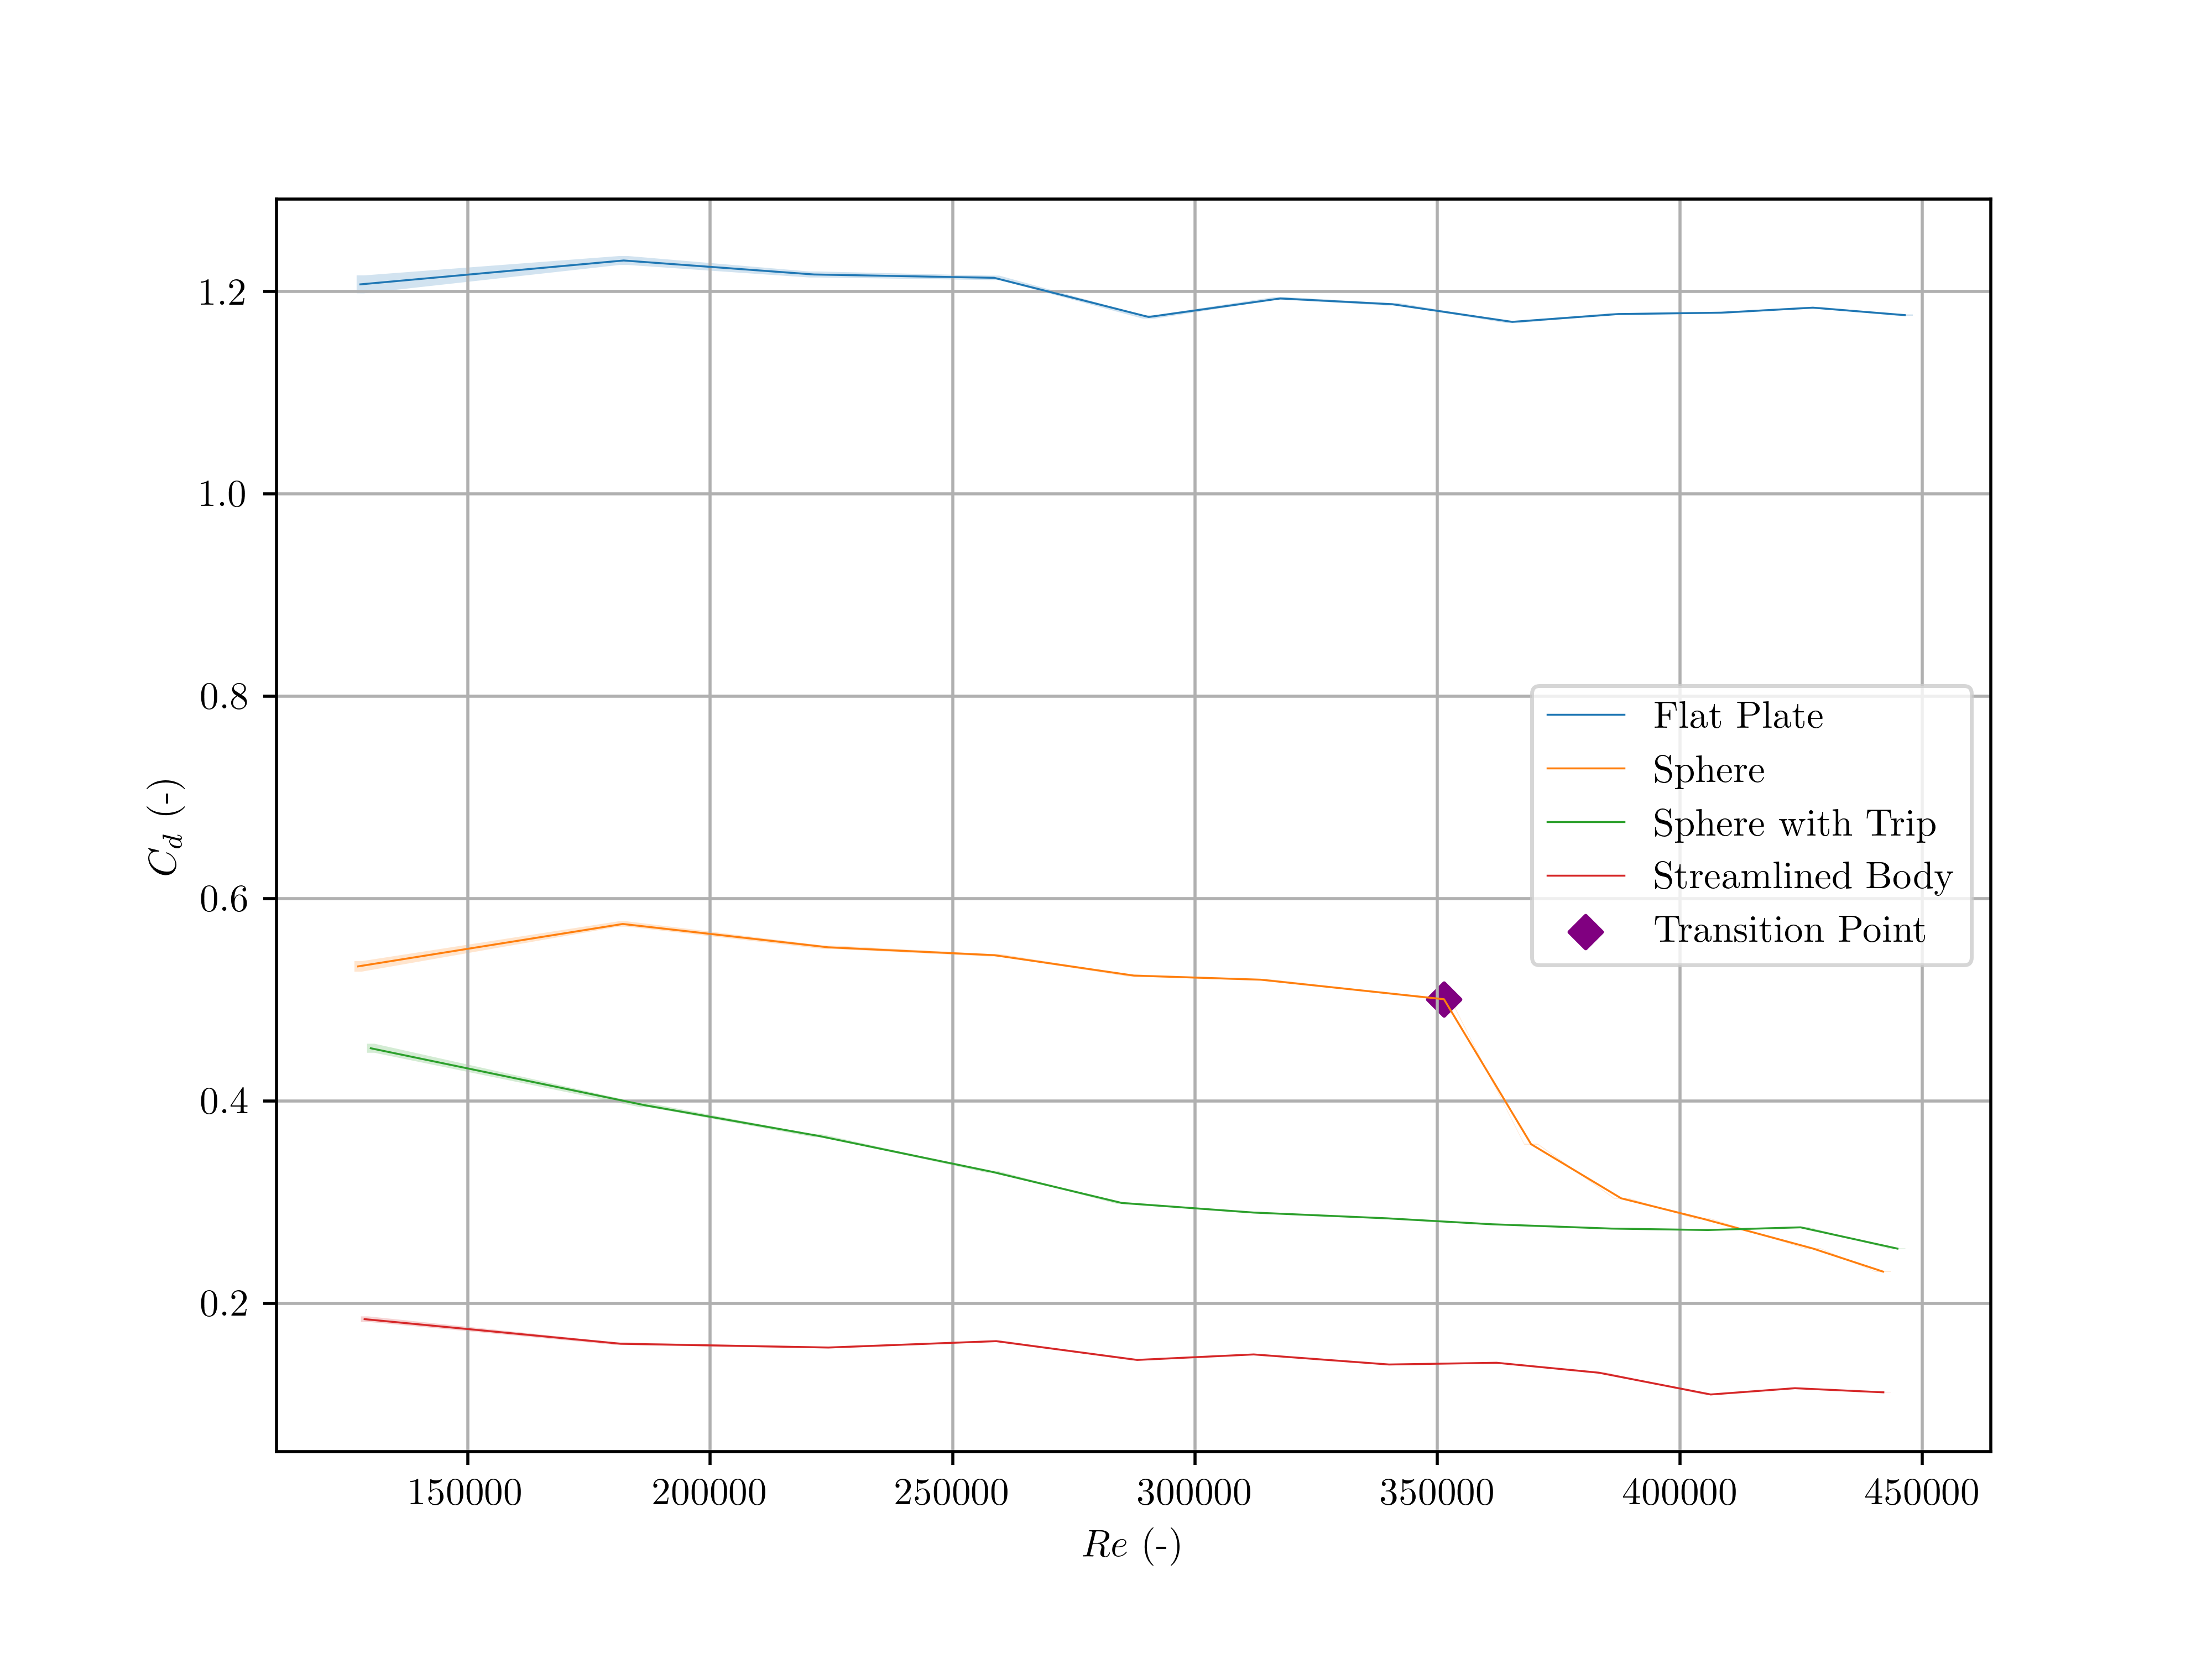
\includegraphics[width=0.8\textwidth]{Re_vs_Cd.png}
    \caption{ReD vs Cd}
    \label{fig:figure1}
\end{figure}

\begin{figure}[H]
    \centering
    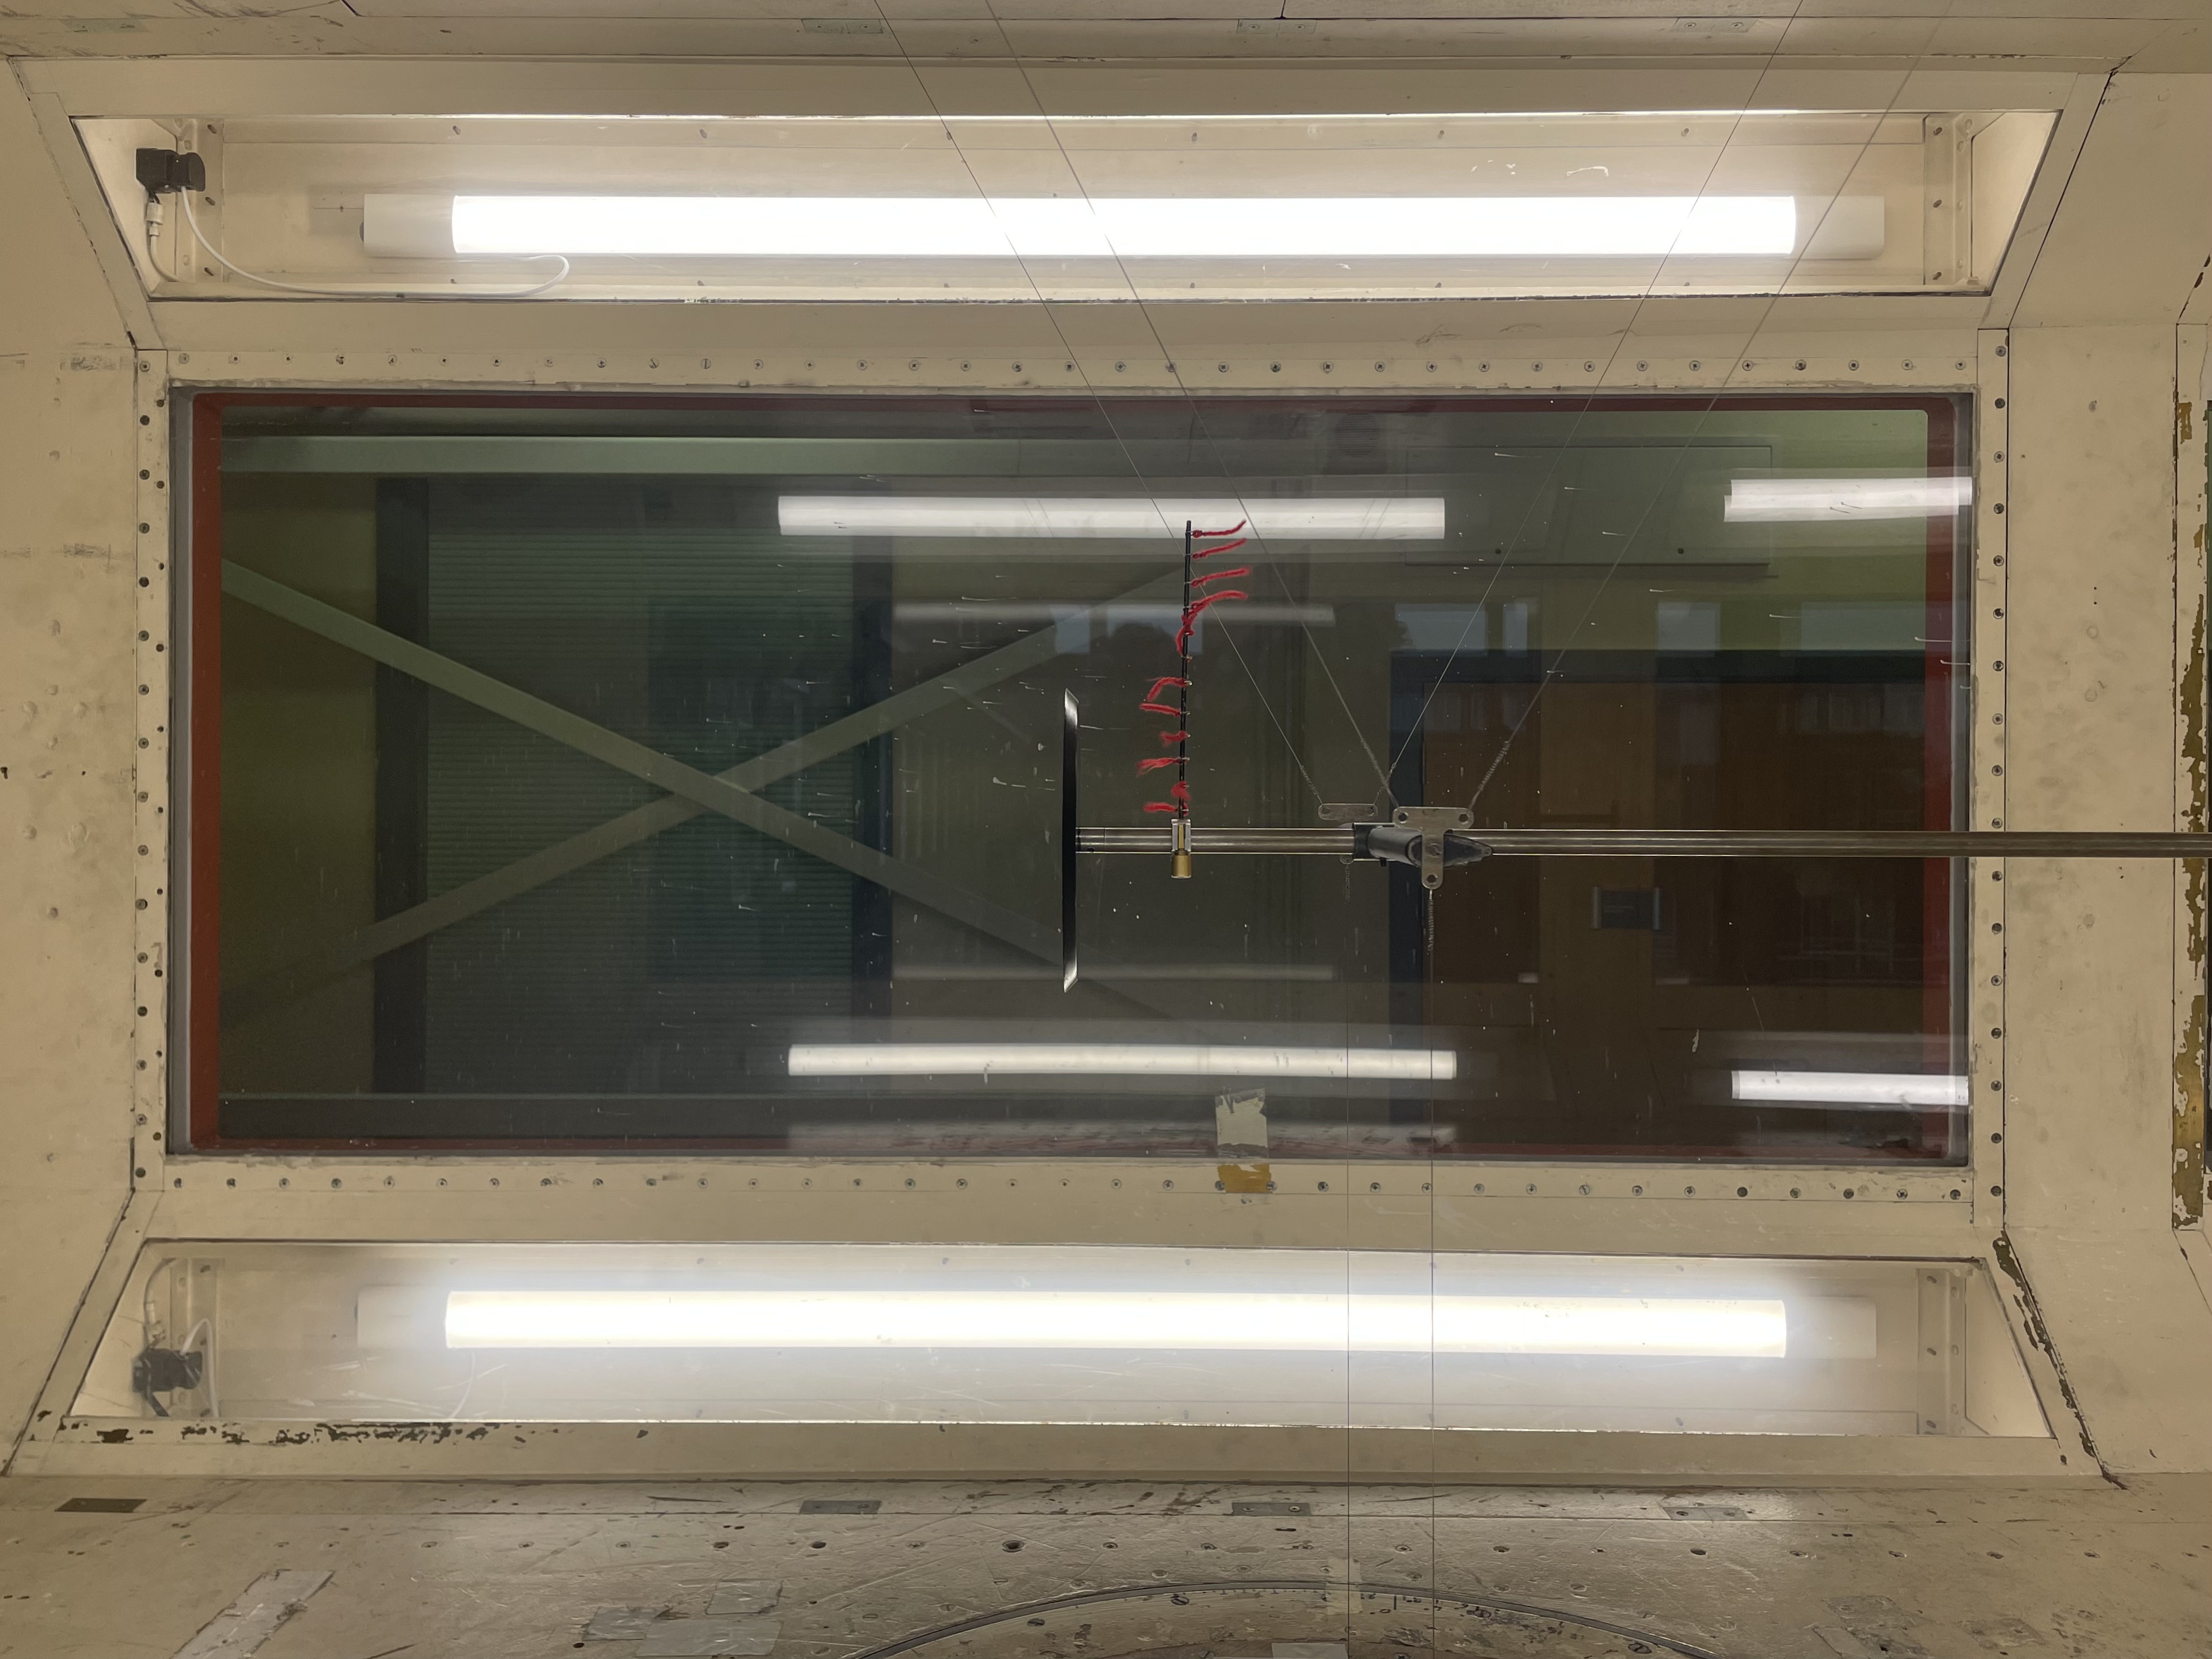
\includegraphics[width=0.8\textwidth]{Images_Videos/Plate_8milibar.JPG}
    \caption{ReD vs Cd}
    \label{fig:figure2}
\end{figure}

\begin{figure}[H]
    \centering
    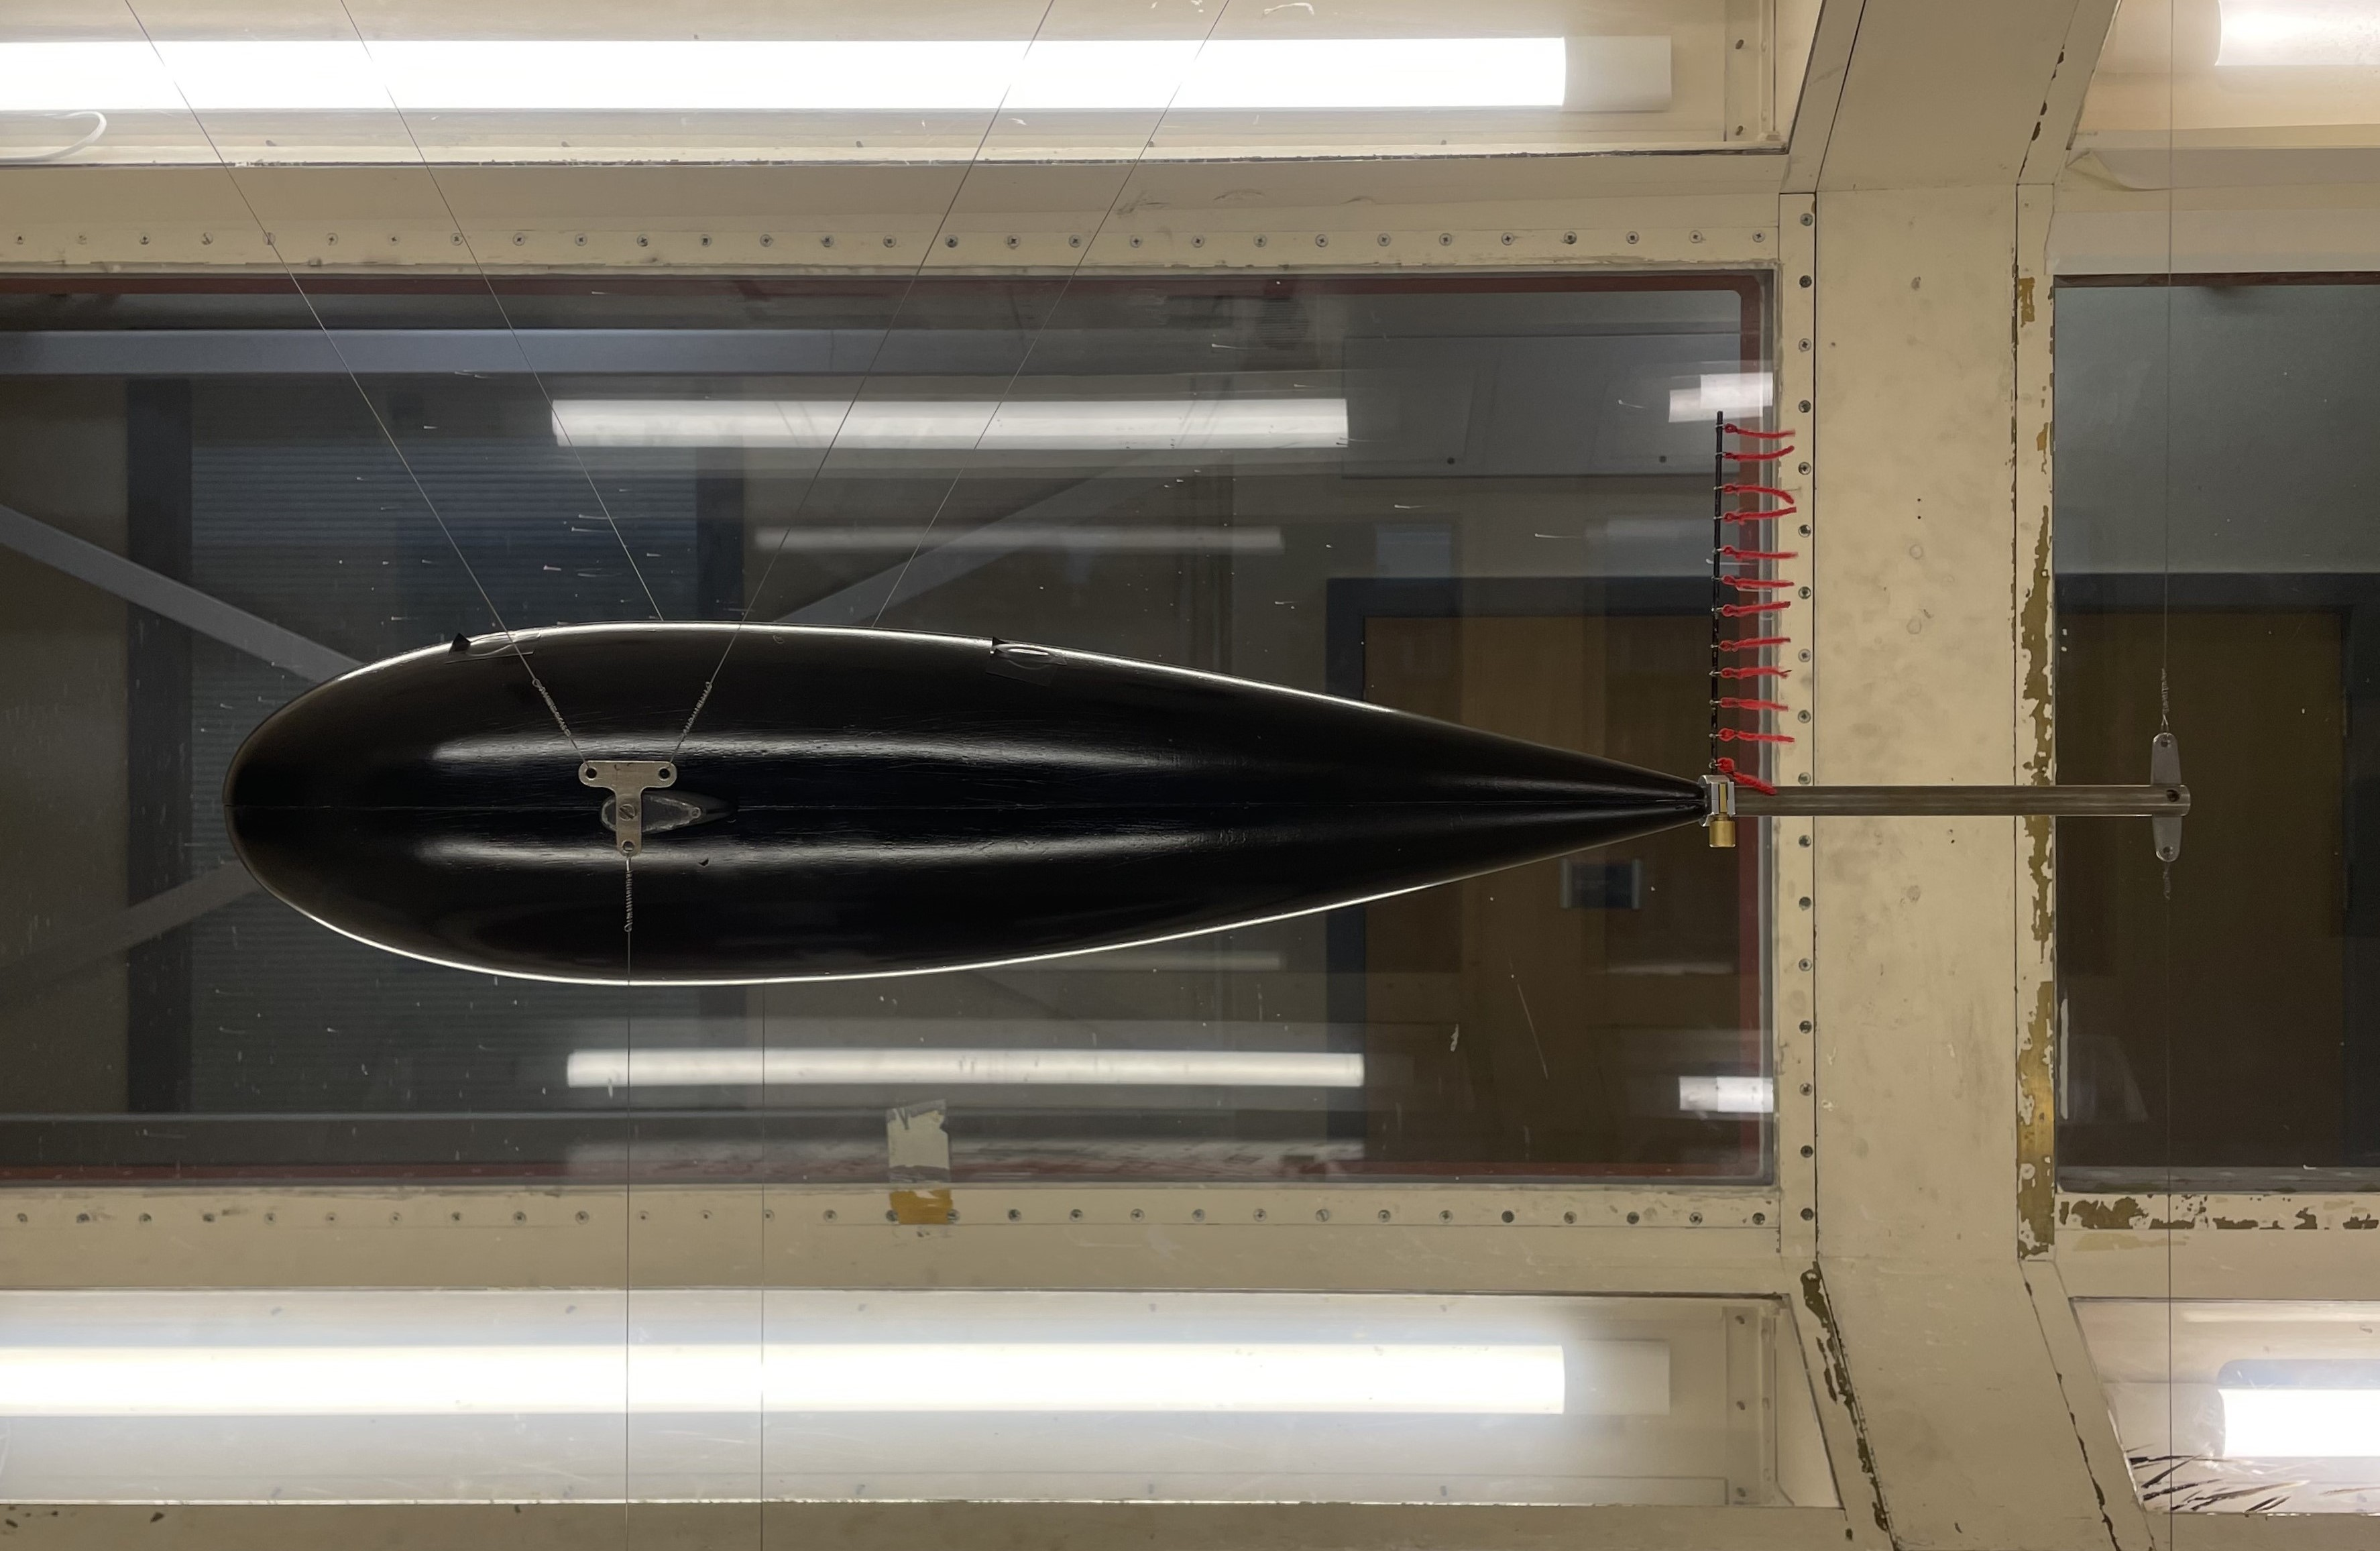
\includegraphics[width=0.8\textwidth]{Images_Videos/Streamlined_8milibar.JPG}
    \caption{ReD vs Cd}
    \label{fig:figure3}
\end{figure}

\begin{figure}[H]
    \centering
    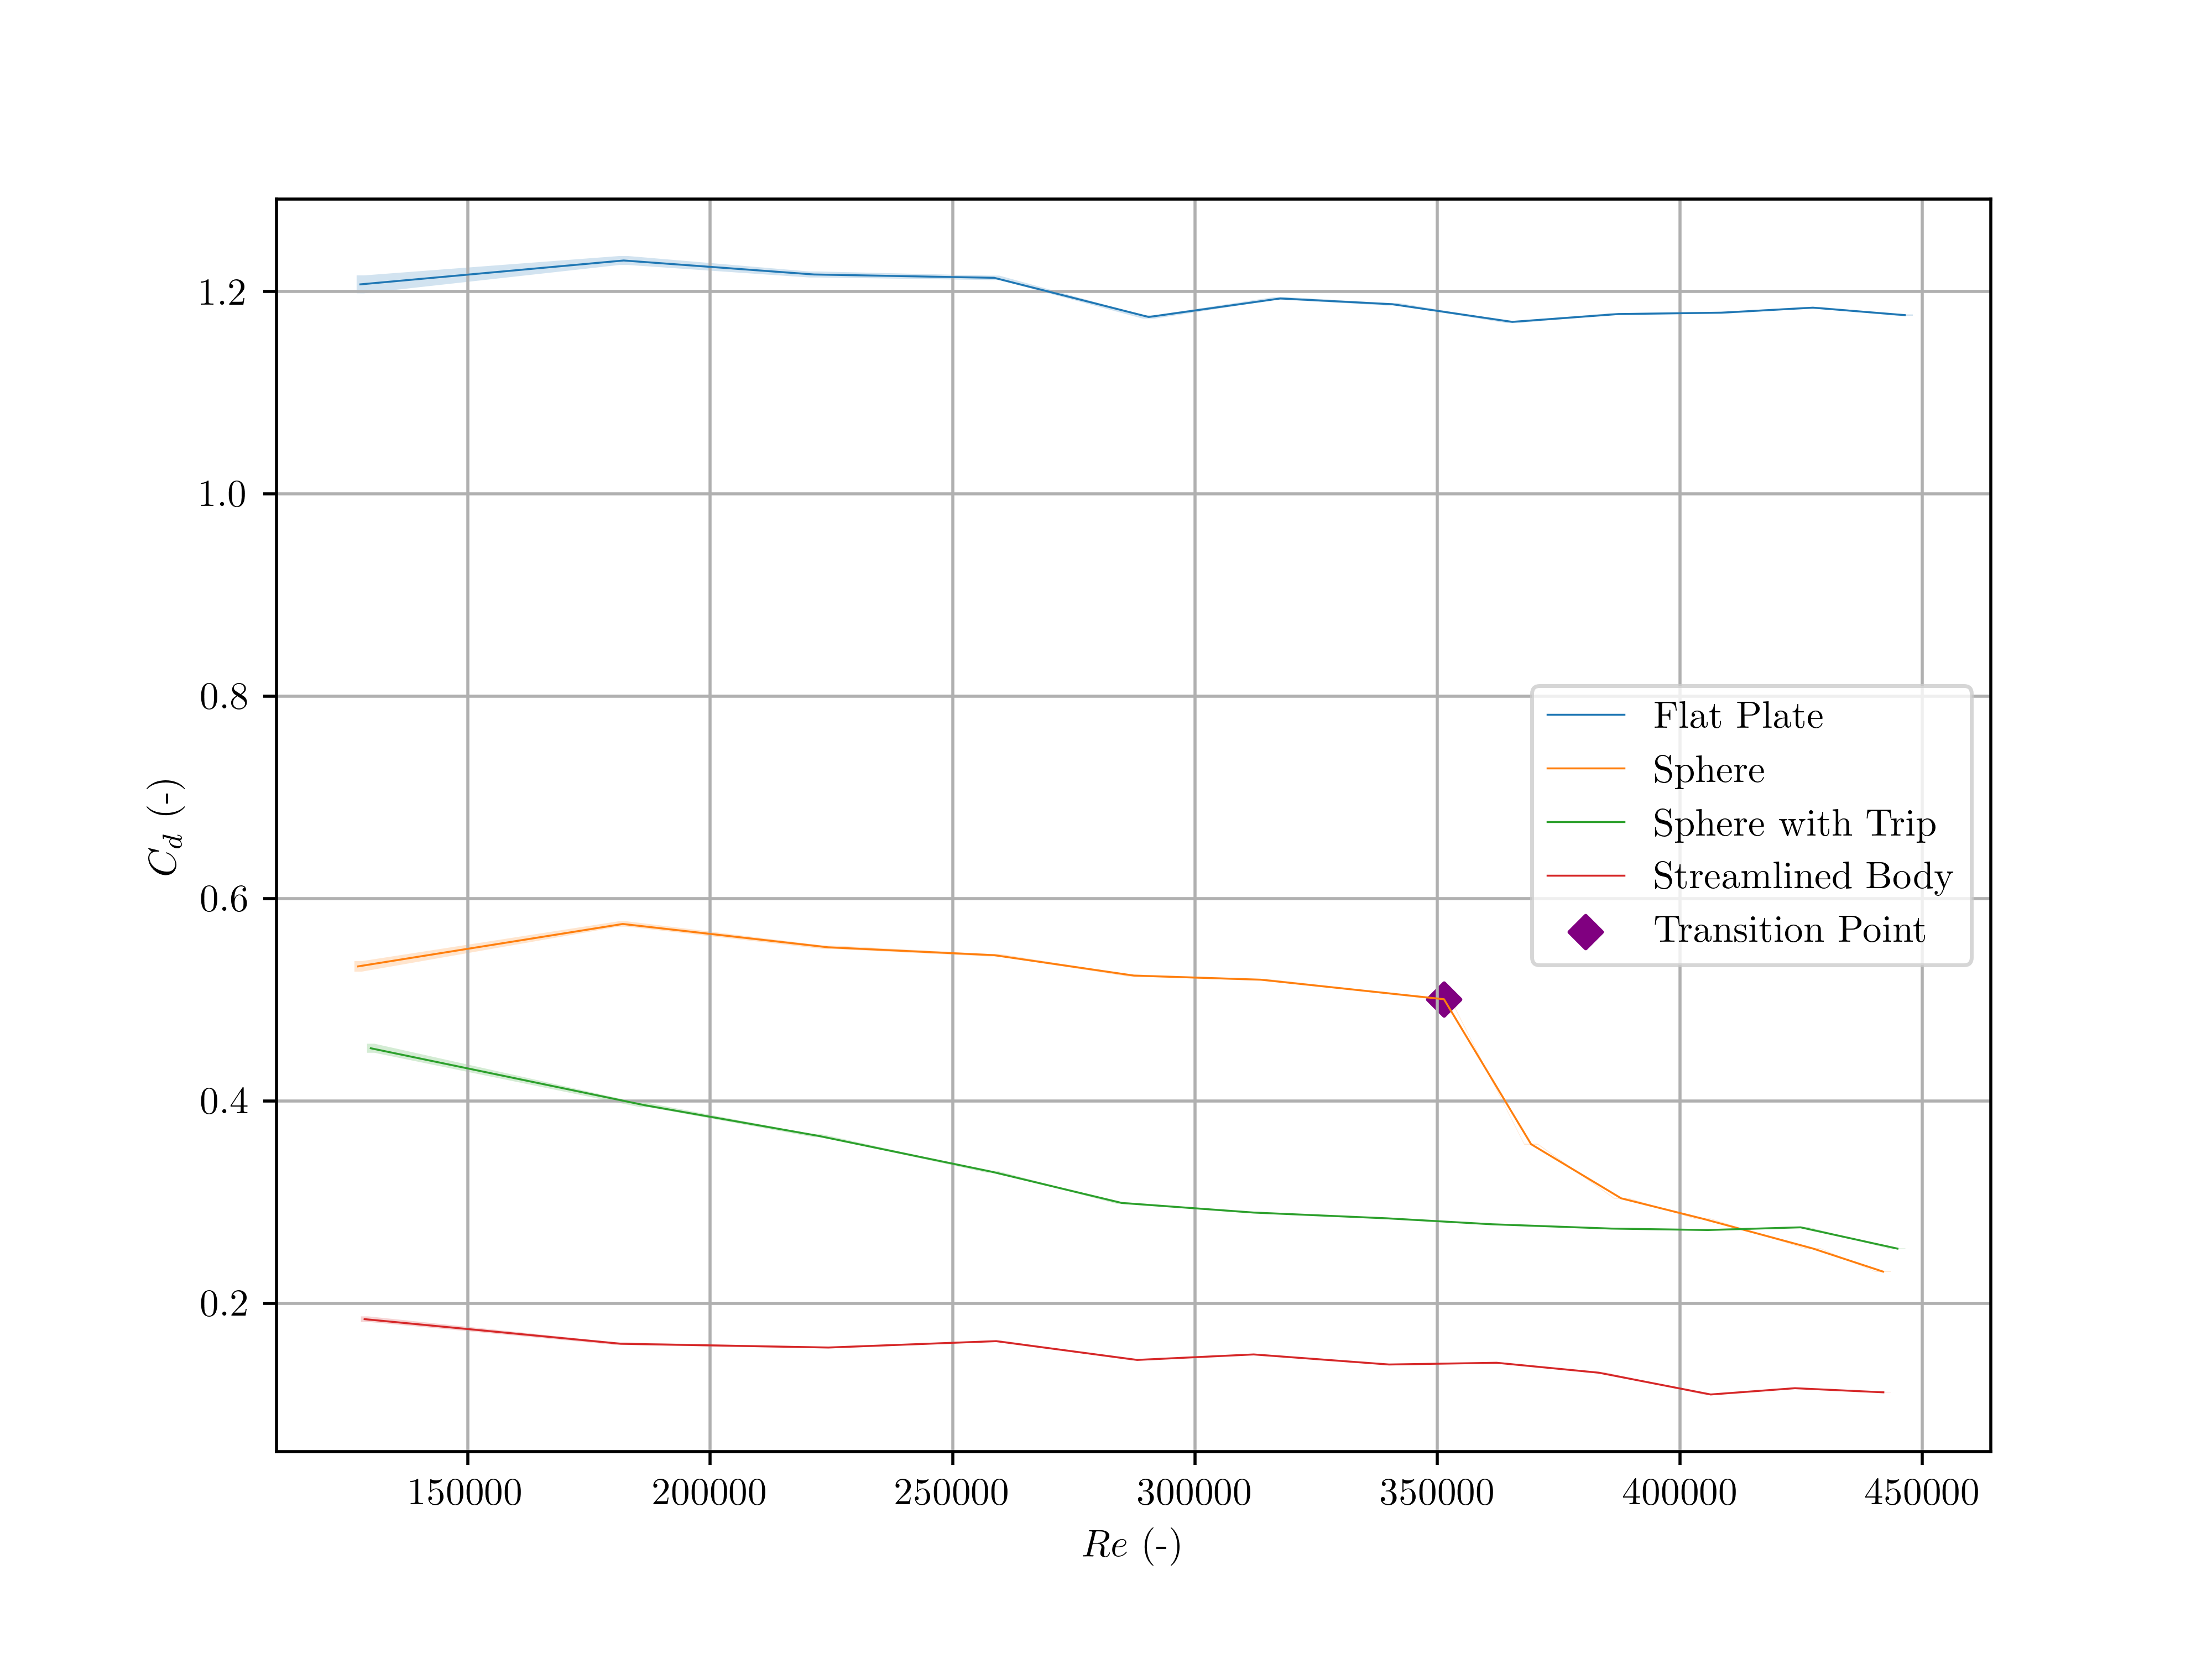
\includegraphics[width=0.8\textwidth]{Re_vs_Cd.png}
    \caption{ReD vs Cd}
    \label{fig:figure4}
\end{figure}

\begin{figure}[H]
    \centering
    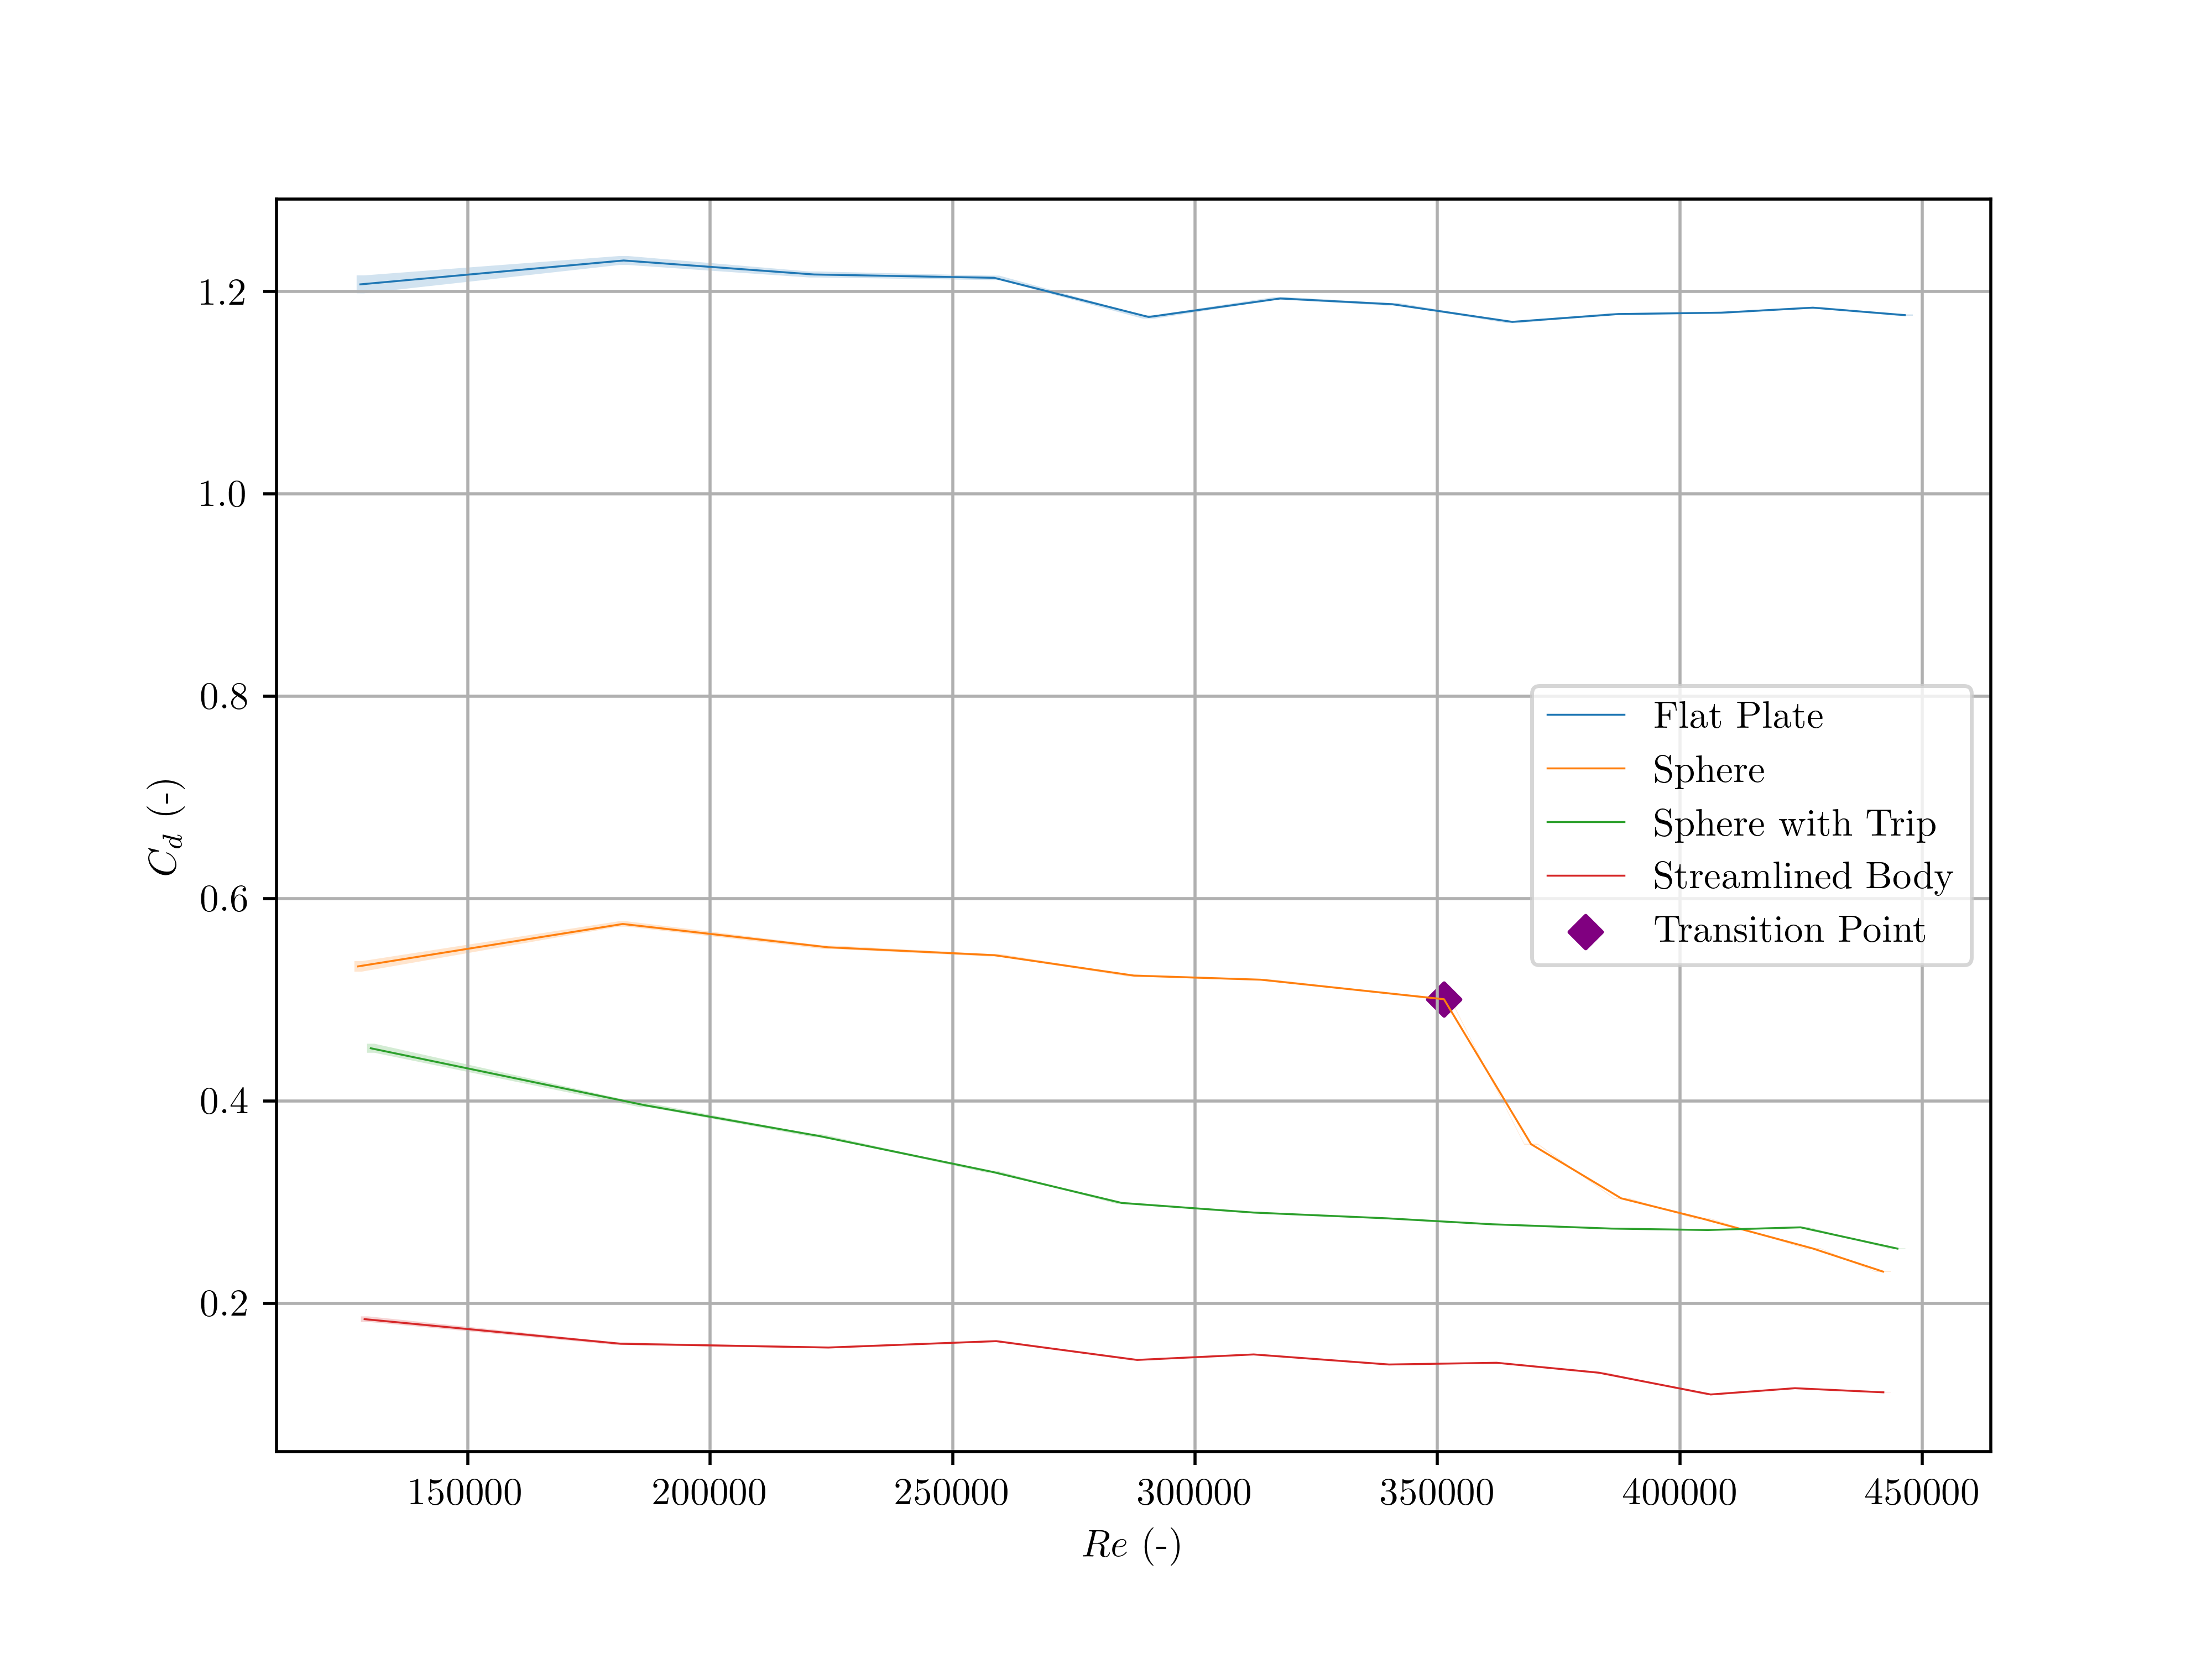
\includegraphics[width=0.8\textwidth]{Re_vs_Cd.png}
    \caption{ReD vs Cd}
    \label{fig:figure5}
\end{figure}

\end{document}
